\subsection{Theory Crafting Next steps}

For the remaining duration, we will focus on three main objectives:
One will be to demonstrate that the \textit{bipolar} colouring
of \textsc{nD-StrongSperner} will keep the reduction parsimonious.
Subsequently, we will demonstrate hardness over the \textsc{\#P} class by finding
reductions from the \textsc{SourceOrExcess} problem due to its separation from $\textsc{\#P}$ as shown in \ref{par:count-ppad}.
And lastly, we aspire to develop enough gadgets and tools to tackle the core question of the project.


\subsection{Software Next Steps}

In the next steps we aim to complete the rest of the milestones. 
We believe that the usage of methods by Eichelberger et al. \cite{eichelberger_HazardDetectionCombinational_1965}
or polynomial algorithms for specific cases of \textsc{PureCircuit} by \cite{deligkas_PureCircuitTightInapproximability_2024}
will allow us to identify solutions.
Although the former method is still exponential in runtime \cite{eichelberger_HazardDetectionCombinational_1965,ikenmeyer_ComplexityHazardfreeCircuits_2019},
we hope its average running time will be sufficient.
Regarding the counting milestone, given the progression of the project, we plan to implement a brute force method
for small instances.

\subsection{Timetable}

Figure \ref{fig:gantt-new} depicts how the remaining project is expected to progress with regard
to the milestones we aim to achieve. Overall we modified our timeline to prioritise
theory crafting, and therefore we hope this adjusted timeline will capture accurately the remaining duration
of the project.

\begin{figure}[h!]
    \centering
    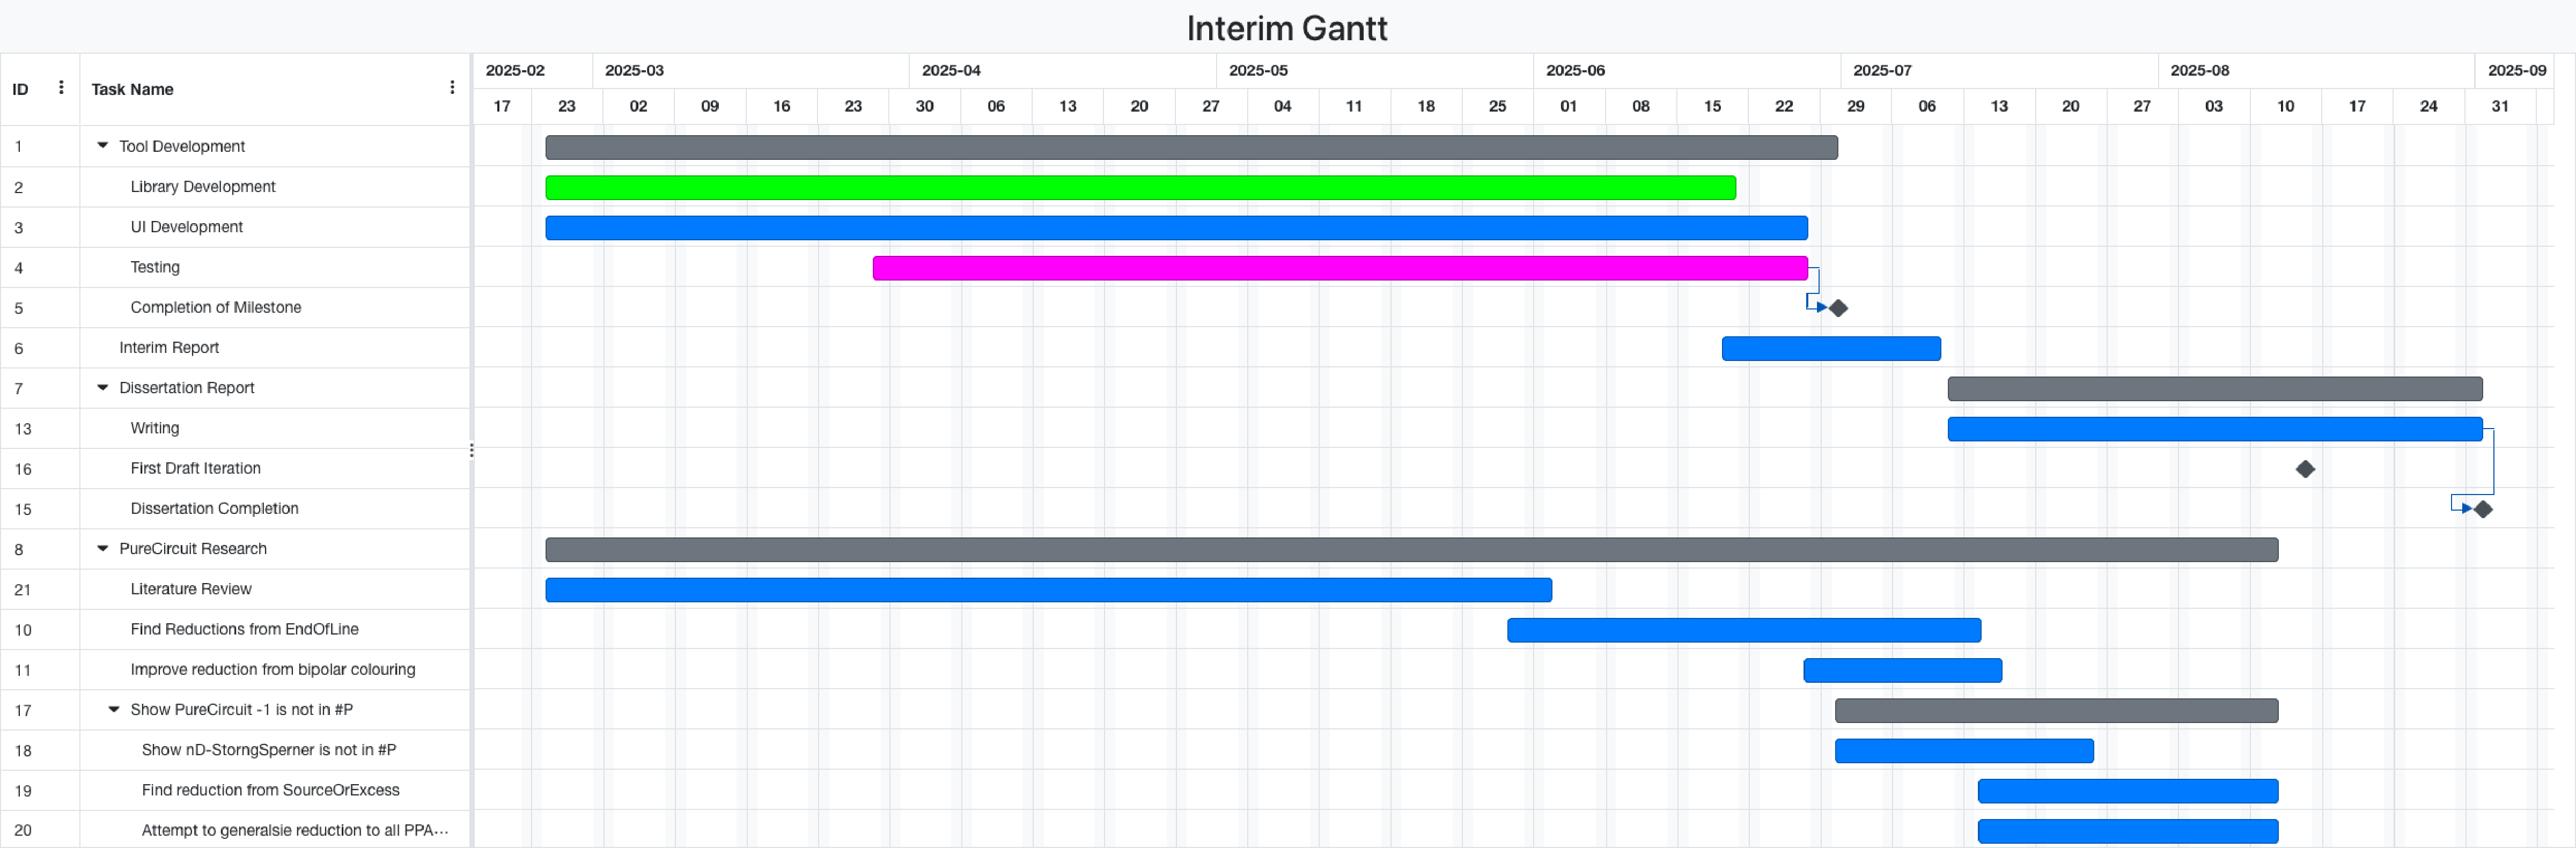
\includegraphics[width=0.85\textwidth]{assets/Interim Gantt 20250708.pdf}
    \caption{Updated Gantt chart}\label{fig:gantt-new}
\end{figure}

